
\documentclass[a4paper,12pt]{article}
\usepackage[a4paper, total={6in, 10in}]{geometry}
\frenchspacing
\usepackage{microtype}
\usepackage{graphicx}
\usepackage{float}
\usepackage{placeins}
\graphicspath{ {./images/} }
\usepackage[pdfauthor={Jenny Vermeltfoort},pdftitle={Model based consistency of variable names for improved high-level understanding.}]{hyperref}
\usepackage[colaction]{multicol}
\setlength\columnsep{30pt}

\usepackage[columnwise]{lineno}
\modulolinenumbers[10]

\usepackage{sectsty}% http://ctan.org/pkg/sectsty
\usepackage{titlecaps}% http://ctan.org/pkg/titlecaps


\usepackage{lmodern}
\fontfamily{lmdh}\selectfont

\usepackage[backend=biber,style=ieee]{biblatex}
\addbibresource{bib.bib}

\begin{document}

\title{Model based consistency of variable names for improved high-level understanding.}
\author{Jenny Vermeltfoort, 3787494}
\date{\today}
\maketitle

\sectionfont{\centering\MakeUppercase}
\begin{multicols}{2}
\linenumbers

\section*{Introduction}
While software is written to be interpreted by computers it is of key importance that developers can quickly understand its semantics. The naming of identifiers is an important tools for software engineers to meaningfully transfer concepts to their colleagues, who might be maintaining, updating, or refactoring the code. Comprehensibility of these concepts might be restricted by the innate free characteristics of naming conventions within software languages. It is therefore of interest to identify what kind of names are difficult to interpret and whether formal rules may support a more meaningful way of transferring concepts.

This report evaluates two research papers that address these issues. The first, written by Floarian Deissenboeck and Markus Pizka, tries to define a formal model to create concise and consistent naming schema in their paper \textit{Concise and consistent naming}.\cite{deisenbock_concise_2005} The second, \textit{Improving Semantic Consistency of Variable Names with Use-Flow Graph Analysis} written by Yusuke Shinyama, Yoshitaka Arahori, and Katsuhiko Gondow develops a probabilistic model to test whether a variable name reflects its intended usage pattern.\cite{shinyama_improving_2021}

This report summarizes, and produces a compounded conclusion of both papers. At the end of the report a short paragraph describes the approach used while writing this report.

\section*{Concise and consistent naming}
Floarian Deissenboeck et al. preamble their paper by describing why bad naming of identifiers is detrimental to the quality of software.\cite{deisenbock_concise_2005} Software engineers are constantly trying to interpret identifier and the concepts they represent. It is therefore important that identifiers meaningfully represent a concept. Identifiers are arbitrarily chosen and the developers often lack a broad understanding of the code base as a whole. When a system evolves, concepts might change or become abandoned; which often leads to improper adaptation of names. These problems damage the coherence of a project and degrade the quality of the code.

According to the authors, meaningfulness does not properly describe why a variable name is good or bad. They divide meaningfulness into two categories, consistency and conciseness. A variable name is consistent when its name only describes one specific concept. When the name is either homonynous or synonymous to multiple concepts it fails this criteria. The word \textit{break} could mean taking a break or could mean breaking a stick. The word \textit{break} thus requires contextualization to fully understand it; which if not done well, becomes ambiguous. Conciseness is determined by the exactness in which a name describes a concept. A example is a hyponym. The word red is a hyponym of the word color, therefore red describes a object more exact then the word color does. The sentence "the red balloon" is more specific than its cryptic counterpart "the colorful balloon".

Most identifiers within the software language are verb-noun compounds, thus identifiers are commonly specialized concepts. The variable \textit{BinaryNodeTree} is a specialized \textit{NodeTree} which in turn is a specialized \textit{Tree}. Two types of compounds are described in the paper, endocentric and exocentric. Endocentric is when a compound is made up of a main and a modifier concept. \textit{School dairy} is a special kind of dairy. Exocentric means that no main concept exists within a compound; is a \textit{television painting} a television or a painting? The authors find that endocentric are the easiest to understand and are therefore the only compound that may be used in software development.

The authors performed analysis on the code base of \textit{Eclipse}, which shows that the source code is made up of 142.275 different identifiers and 11.482 different atomic words; also atomic words are often written in different manners (\textit{frag, fragment, fragments, etc}). According to Deissenboeck et al. this is detrimental to the cohesion of the project. Analysis of the project \textit{CloneDetective} shows that code decay occurred over time. Many identifiers were not adapted after code refactoring and as a result some identifiers do not represent the implementation. Analysis of more projects show similar results.

The authors have developed a half automated tool for Java developers. The tool, a plugin for Eclips IDE, is a identifier dictionary which presents popups and allows auto-completion when creating variable names. It also can perform automated refactoring of already existing code. The tool lessens efforts needed to comply with naming rules. The authors seem interested to see how their model works for other mid to large scale code bases.

\section*{Improving Semantic Consistency}
Yusuke Shinyama et al. find that the semantic consistency of variable names is an important factor for high level understanding of repositories.\cite{shinyama_improving_2021} In their paper they define an automated method to identify and correct name inconsistency’s over a project. The method is based upon a multitude of research papers; which, in short, conclude that long descriptive names improve understanding and that inconsistent naming results in a decay of code quality.

A multitude of researchers have grasped at the problem of identifying consistency of identifier. One converts source code in word embedding and relates it to the natural language, another uses manually crafted rules to detect naming bugs, and another validates whether method names properly describe the method’s code contents. Shinyama et al. use a novel approach by trying to identify semantic inconsistency of variable names by comparing the relations of variable names to their contexts. Their model does not only look at method names but also at variable names, which accordingly, better infer the project’s high-level design.

The consistency of a identifier may be determined by placing the variable name within its context. Code implements a set of operations on a variable, this set of operations is considered the context of a variable name; it is the relation of the name towards its usage. A concrete relationship for every variable name towards its concept is established. Then through comparison the consistency of each identifier may be predicted. 

For illustration purposes see the example of a variable name and its context below. 
\fontsize{7pt}{7pt}\selectfont
\begin{verbatim}
    int year_birth = get_time_person(person).year;
    int age = calc_age(year_now, year_birth);
\end{verbatim}
\fontsize{12pt}{12pt}\selectfont

The variable name “year\_birth” may be substituted by an arbitrary name “x”. The initial assignment using the method call \textit{get\_time\_person} and the designation method call \textit{calc\_age} form the context for variable "x". The following code snipped thus describe the relation of the variable “x” to its context. 
\fontsize{7pt}{7pt}\selectfont
\begin{verbatim}
    int x = get_time_person(person).year;
    int age = calc_age(year_now, x);
\end{verbatim}
\fontsize{12pt}{12pt}\selectfont
By comparing all the variable names that fit within a simular relation, consistency may be determined for any variable within the project.

To support automation of this process the paper proposes a graph structure -- a “Use-Flow Graph” (UFG) -- to describe the context of a variable. See the figure below. The graph depicts the origin, the operations and the designation of the variable. By traversing the lanes from top to bottom for each variable an usage pattern is constructed. This usage pattern  may be used for consistency analysis as described in the paragraphs before. Certain software specific operations -- in this example the mathematical operators -- are depicted using unique blocks; think of \textit{while}- and \textit{for}-loops, \textit{if}-statements, and method calls. 

\begin{figure}[H]
    \centering
    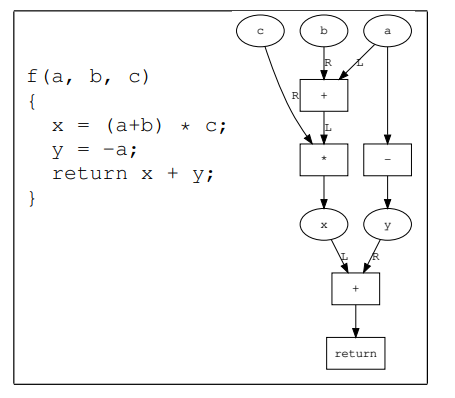
\includegraphics[width=1.0\linewidth]{ufg}
    \caption{example UFG. A copy of fig. 3.\cite{shinyama_improving_2021}}
    \label{fig:ufg}
\end{figure}
\hfill

Experiments using their model were performed on a couple of projects. The goal of the experiments was to proof that the model produces a name that accurately describes the usage pattern. A part of the experiment was asking nine independent reviewers, being uninformed by the name's origin, whether they preferred the original name, the name produced by the model, or the name produced by a different model. Results show that the reviewers moderately agreed that the identifiers produced by the authors' model where the best; results where based on the Fleiss' Kappa scale.
    
The paper shows that the automated method defined by the paper is capable of providing improved consistent naming schema within a project. However, the authors note a clause concerning the results; the small pool of nine reviewers might be biased which could have skewed the results; also the method is only designed for Java code and software languages with dynamic dispatch and variable aliasing exceed the model's limitations.

\section*{Conclusion}
Both papers seemingly agree that the consistency of a variable names depends on its usage pattern; a variable has to correctly describe its indented concept. It is interesting to see how each paper tackles the problem of name consistency in a different manner. Deissenboeck et al. offer an formal, more abstract, model on providing guidelines for consistent and concise naming conventions.\cite{deisenbock_concise_2005} While Yusuke et al. have produced a precise and consistent way to determine the consistency of a identifier by their usage pattern; thus restricting the scope of the model to the specific project of the identifier.\cite{shinyama_improving_2021}

Deissenboeck et al. partially base their findings on \textit{Software psychology} written by Shneiderman that states that meaningful names are an important factor for better understanding of complex systems.\cite{schneiderman_software_1980} Deissenboeck et al. expand this conclusion by interpolating the word \textit{meaningful} over a couple of concrete rules which constitute their model.\cite{deisenbock_concise_2005} The paper however merely show the model being used for analysis and does not present any statistical argumentation for why the model improved understanding. It is therefore inconclusive whether their model actually improved the semantic understanding for any of these projects. In contrast the experiments performed by Yusuke et al. on their model is quite extensive and, albeit limited in execution, the results at least support their conclusion. 

Purely looking at the conclusions of these two papers there seem to exist a relative weakness that arises from researching a subjective topic. The problem with these two papers is that there seems to be a lack of foundational understanding of what consistency means within the framework of identifiers, since both papers define consistency in a different manner. While some formal rules may improve cohesion of software development overall, it seems almost impossible to define some objectively most efficient schema that projects an identifiers meaningfulness. Possibly this gap might be bridged by integrating recent psychological or linguistic research into future research of this topic.


\section*{Assignment approach}
Firstly I analysed the assignment and developed a high-level plan. This entails that I wrote a small section of the introduction and predefined the sections. 

Secondly I tried to find an academic paper related to the topic. I used a couple of databases, Leiden University Librarie Catalogue and Google Scholar. Found an older paper written by Deissenboeck et al. in 2005, the article itself and a broad selection of Deissenboeck's papers are highly influential according to Semantic Scholar. The paper written by Yusuke et al. is less influential, however it is much more recent (2022). Yusuke et al. have all written a plethora of papers related to the topic and their references used within the article are quite influential. 

Thirdly I read both papers and made notes and highlights along the way. Then I summarized each paper individually. I struggled with finding the right balance when it came to descriptiveness and conciseness. So I made a quick map with short item descriptions for each paper that I wanted to be part of the summary. It allowed me to keep things comprehensible and logically sequenced. 

Fourthly I wrote the conclusion, which I formulated from some notes that I made while reading. While I was reading I had some doubts about certain arguments and thought of things that were missing. I also thought about how I would tackle the problem.

At last, I rewrote multiple parts to improve the cohesion and overall flow of the text.

\end{multicols}

% the bibliography
\printbibliography

\end{document}

